\documentclass[11pt,letterpaper]{article}
\usepackage[margin=1in]{geometry}
\usepackage{graphicx,booktabs,tabularx,array,xcolor,amsmath,enumitem,titlesec,fancyhdr}
\usepackage[hidelinks]{hyperref}
\usepackage[most]{tcolorbox}

\definecolor{accent}{HTML}{1F3A5F}
\titleformat{\section}{\large\bfseries\color{accent}}{\thesection.}{0.5em}{}
\titleformat{\subsection}{\normalsize\bfseries}{}{0em}{}
\setlist{itemsep=2pt,topsep=4pt}
\setlength{\parskip}{5pt}\setlength{\parindent}{0pt}
\pagestyle{fancy}\fancyhf{}\renewcommand{\headrulewidth}{0pt}
\fancyfoot[L]{\small\color{gray}Canadian Credit Relative Value}\fancyfoot[R]{\small\color{gray}\thepage}
\newcolumntype{Y}{>{\raggedright\arraybackslash}X}

\begin{document}

{\color{accent}\LARGE\bfseries Canadian Credit Relative Value}\\[4pt]
{\large Finding cheap and rich Canadian investment-grade corporate bonds, and testing whether the gaps close}\\[8pt]
{\small Esther Wong \quad$\cdot$\quad October 2026 \quad$\cdot$\quad Data as of September 30, 2026}

\vspace{6pt}
\begin{tcolorbox}[colback=accent!5,colframe=accent,boxrule=0.6pt,arc=2pt,title=\textbf{Key results},fonttitle=\small]
\small
\begin{itemize}[leftmargin=12pt]
  \item \textbf{Universe:} 233 Canadian-dollar senior unsecured bonds from 15 issuers (banks, telecom, pipelines, utilities), 45 month-ends from January 2023 to September 2026.
  \item \textbf{Model:} issuer and sector spread curves plus a fundamental regression; monthly $R^2$ of 0.87--0.96, driven mostly by rating and sector.
  \item \textbf{Structure matters:} within the same issuer, premium bonds trade up to $\sim$2.5bp wider per price point and bank notes callable a year early $\sim$20bp wider. Without correcting for this, ``cheap'' simply meant ``high coupon''.
  \item \textbf{Signal:} the cheapest fifth of bonds beat the richest by $\sim$3bp per quarter in every year tested (Fama-MacBeth $t \approx -6$); mispricings close with a half-life of about 8--12 months.
  \item \textbf{Trade:} long Pembina 3.62\% 2029 / short TCPL 3.00\% 2029, CS01-neutral. The model expects +9.9bp over 12 months; after real bid/ask and borrow costs it is roughly breakeven, so the trade is a hold with a $\sim$29bp entry threshold.
\end{itemize}
\end{tcolorbox}

\section{Objective}
Bonds from issuers with similar credit quality often trade at different spreads. Credit desks look for these gaps because they tend to close. This project measures those gaps across the Canadian investment-grade corporate market, tests whether they close, and turns the strongest one into a trade a desk could act on.

\section{Data}
The model is built from free, public sources behind one common data format, so a Bloomberg feed could replace any of them without changing the model.

\begin{center}\small
\begin{tabularx}{\linewidth}{@{}l Y Y@{}}
\toprule
Need & Source & Notes \\
\midrule
Bond list, prices, terms & iShares XCB month-end holdings (BlackRock Canada) & $\sim$1,350 holdings per month; ISINs joined from a second file (100\% match) \\
Government of Canada curve & Bank of Canada Valet API & 2, 3, 5, 7, 10-year and long benchmarks \\
Leverage and coverage & SEC EDGAR filings (40-F, 10-K, 20-F) & First-filed values with filing dates, so no look-ahead \\
Credit ratings & Annual Information Forms on EDGAR & 98 dated S\&P / Moody's / DBRS ratings, each checked against a verbatim quote \\
\bottomrule
\end{tabularx}
\end{center}

\textbf{Universe.} Canadian-dollar, senior unsecured, fixed-coupon bonds with 2--12 years to workout in four sectors. Three things a terminal screen would have labelled had to be detected from the data:
\begin{enumerate}[leftmargin=16pt]
  \item \textbf{Bank subordinated debt} appears under the bank's plain name; bonds with $\sim$10-year terms (NVCC, 10NC5) were excluded.
  \item \textbf{Callable bank senior is now the norm.} Since 2023 the big banks issue bail-in senior as 4NC3, 5NC4 and 6NC5 notes; these are priced to the call date, as the market quotes them.
  \item \textbf{Floating-rate notes} appear with their current coupon and were excluded.
\end{enumerate}
Callables and floaters were found by comparing the ETF's reported duration with the duration implied by a plain bullet bond. After the fixes, every bond's computed duration matches the ETF's (median gap 0.03 years).

\textbf{Spreads.} Yields are computed from clean prices (semi-annual, Actual/365 accrual) to each bond's workout date. The G-spread is the bond's yield minus the Government of Canada yield interpolated to the same maturity. Median spreads tightened in every sector over the sample (Table~\ref{tab:spreads}), so the backtest covers one long rally.

\begin{table}[h]\centering\small
\caption{Median G-spread by sector (bp)}\label{tab:spreads}
\begin{tabular}{@{}lrrrr@{}}\toprule
 & Banks & Pipelines & Telecom & Utilities \\ \midrule
2023 & 112 & 172 & 164 & 132 \\ 2024 & 70 & 125 & 120 & 102 \\ 2025 & 69 & 110 & 105 & 87 \\ 2026 & 68 & 94 & 84 & 74 \\ \bottomrule
\end{tabular}
\end{table}

\section{Structural effects: coupon, age and calls}
A first version of the issuer curves flagged every 6--8\% coupon bond as cheap and every 2--3\% coupon bond as rich; price premium alone explained 39\% of the curve residuals. Bonds of the same issuer share credit risk, so systematic spread differences between them are structural. Each month, residuals from the issuer curves were regressed on three bond characteristics (Table~\ref{tab:struct}).

\begin{table}[h]\centering\small
\caption{Within-issuer structural effects (median by year)}\label{tab:struct}
\begin{tabularx}{\linewidth}{@{}l rrrr Y@{}}\toprule
Effect & 2023 & 2024 & 2025 & 2026 & Likely cause \\ \midrule
bp per point of price above par & 1.0 & 1.4 & 1.9 & 2.5 & Tax treatment favours discount bonds \\
bp per ln(1 + years since issue) & 9.1 & 9.0 & 6.0 & 1.6 & Older bonds are less liquid \\
bp for a 1-year-early call & -- & 30 & 20 & 14 & Call and extension risk on bank notes \\ \bottomrule
\end{tabularx}
\end{table}

Every spread is then converted to a \textbf{par-equivalent spread}: what a par-priced, newly issued bullet of the same issuer would trade at. After the adjustment, residuals have essentially zero correlation with price premium. One pattern survives all controls: low-coupon bonds issued in 2020--21 (e.g.\ TCPL 2.97\% 2031, Enbridge 2.82\% 2031, TELUS 2.85\% 2031) still look rich as a group, so the trade step only pairs bonds of similar price and vintage.

\section{Method}
\subsection{Spread curves}
Each month, par-equivalent spread $= a + b \ln(\text{years to workout})$ is fitted per issuer (4+ bonds) and per sector. Each bond is judged against the curve fitted on its \emph{other} bonds (leave-one-out, $e_i/(1-h_{ii})$), because with 4--10 bonds per issuer an in-sample fit pulls toward the bond itself. Residuals become robust z-scores, and a bond is flagged when it is beyond $\pm1.5\sigma$ on both its issuer and sector curve (about 14 bonds per month).

\begin{figure}[h]\centering
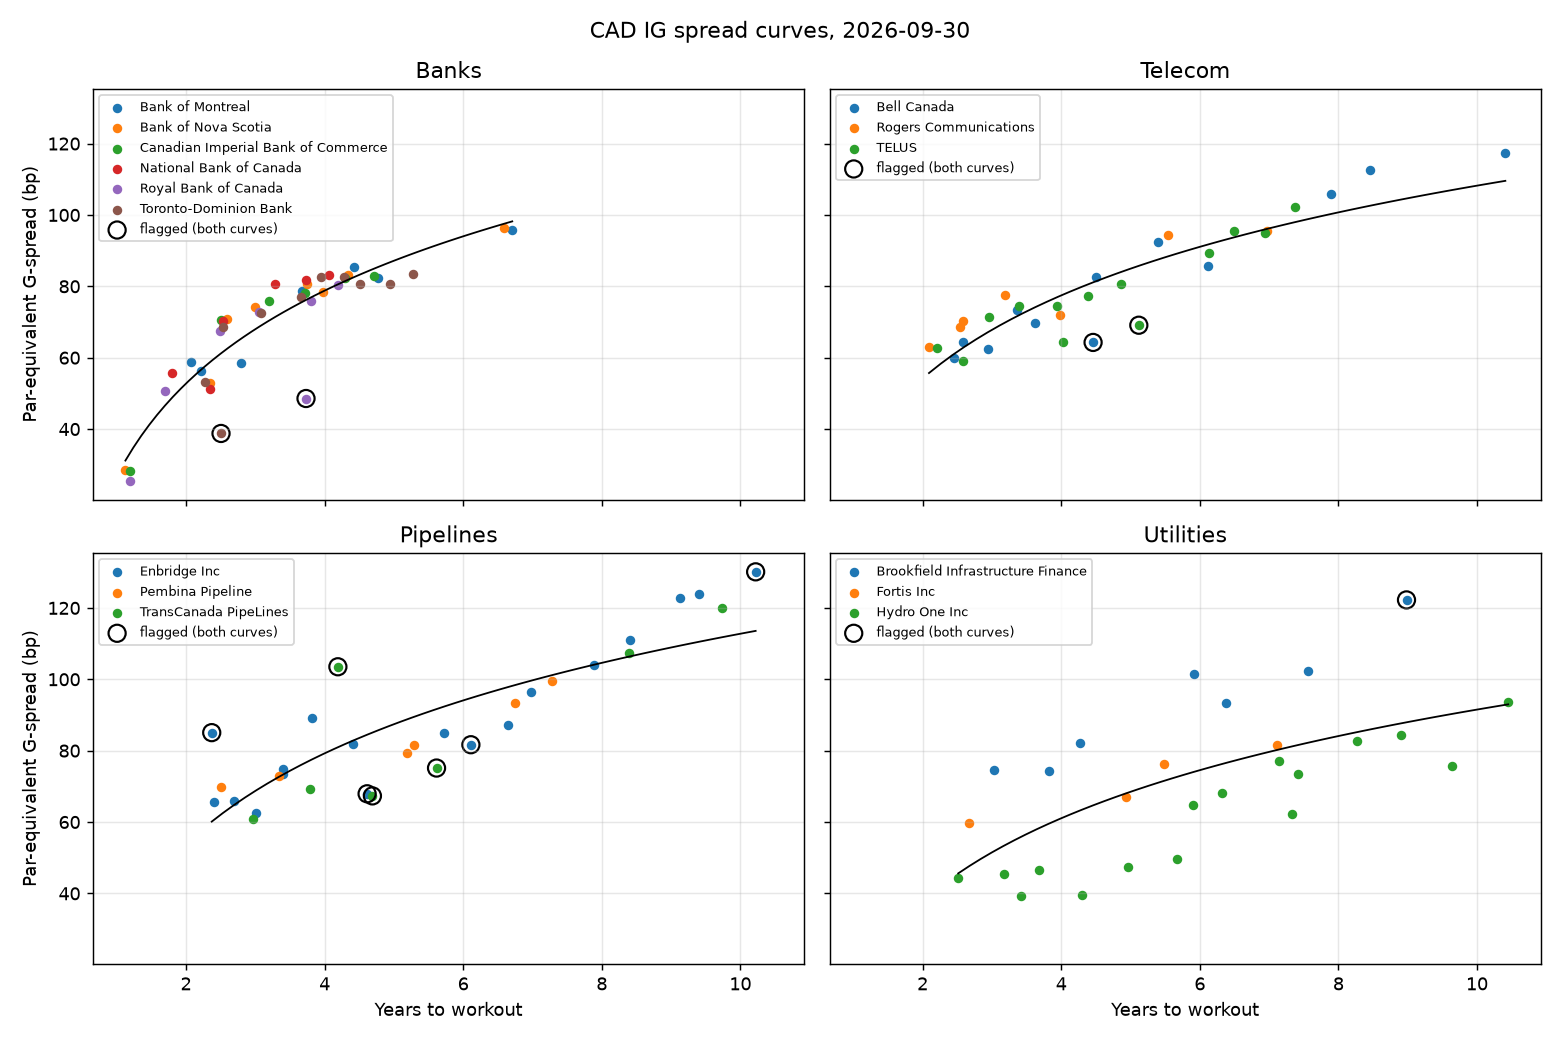
\includegraphics[width=0.92\linewidth]{figures/sector_curves_2026-09.png}
\caption{Par-equivalent spread curves by sector, September 2026. Circled bonds are flagged on both curves.}
\end{figure}

\subsection{Fundamental regression}
\[
\text{G-spread}_i = \alpha + \beta_1 \ln T_i + \beta_2\,\text{Rating}_i + \beta_3\,\tfrac{\text{Net debt}}{\text{EBITDA}}_i + \beta_4\,\text{Coverage}_i + \beta_5 \ln \text{Size}_i + \text{controls} + \gamma_{\text{sector}} + \varepsilon_i
\]
Controls are price premium, bond age, a callable flag and a bail-in flag; banks enter with zero leverage and coverage and a sector dummy. A monthly cross-section produces the point-in-time signal; a pooled panel with month fixed effects and issuer-clustered standard errors gives the coefficients (Table~\ref{tab:reg}).

\begin{table}[h]\centering\small
\caption{Pooled panel regression of G-spread (bp), $n = 4{,}708$ bond-months, 12 issuers}\label{tab:reg}
\begin{tabular}{@{}lrrrr@{}}\toprule
Variable & Coef. & Clustered SE & $p$ & Same sign monthly \\ \midrule
ln(years to workout) & 52.5 & 2.6 & $<$0.001 & 100\% \\
Rating (per notch worse) & 5.8 & 1.6 & $<$0.001 & 96\% \\
Net debt / EBITDA & 1.6 & 1.6 & 0.33 & 53\% \\
EBITDA / interest & $-$0.2 & 0.9 & 0.86 & 53\% \\
ln(size) & $-$4.0 & 2.1 & 0.05 & 96\% \\
Price premium (per point) & 1.5 & 0.2 & $<$0.001 & 100\% \\
ln(1 + age) & 7.3 & 2.2 & 0.001 & 87\% \\
Callable a year early & 20.5 & 4.1 & $<$0.001 & 100\% \\
Bail-in vs legacy senior & 30.9 & 3.5 & $<$0.001 & -- \\ \bottomrule
\end{tabular}
\end{table}

Monthly $R^2$ ranges from 0.87 to 0.96. That should not be oversold: with 12 issuers, rating and sector nearly pin down each issuer's average spread. \textbf{Leverage and coverage are not significant}; seven non-bank issuers are too few to separate them from rating and sector. A bond is a final cheap or rich signal only when the regression and both curve fits agree beyond $\pm1.5\sigma$ (about 9 bonds per month).

\begin{figure}[h]\centering
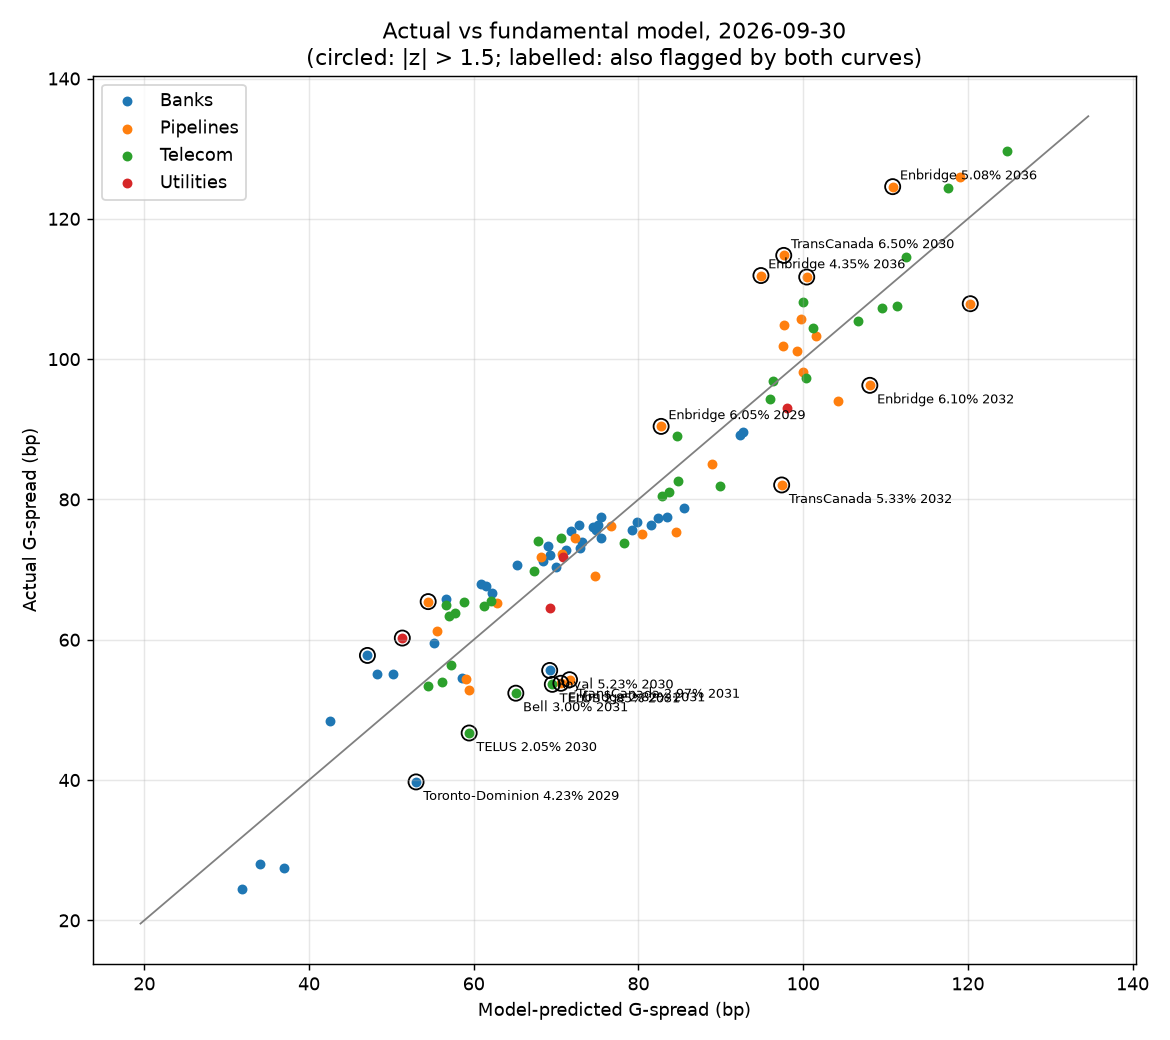
\includegraphics[width=0.62\linewidth]{figures/actual_vs_model_2026-09.png}
\caption{Actual vs model-predicted G-spread, September 2026.}
\end{figure}

\section{Backtest: do the gaps close?}
Every month, using only information available at the time, each bond's residual is compared with its \emph{excess} spread change over the next 1--3 months: its own change minus its sector's average, net of roll-down.

\begin{table}[h]\centering\small
\caption{Fama-MacBeth slope of forward excess spread change on today's residual (Newey-West $t$)}
\begin{tabular}{@{}lrrr@{}}\toprule
Residual & 1 month & 2 months & 3 months \\ \midrule
Regression & $-$0.045 ($-$6.4) & $-$0.075 ($-$6.0) & $-$0.102 ($-$5.3) \\
Issuer curve & $-$0.026 ($-$3.5) & $-$0.042 ($-$2.9) & $-$0.058 ($-$2.7) \\
Sector curve & $-$0.027 ($-$4.0) & $-$0.046 ($-$3.7) & $-$0.065 ($-$3.6) \\ \bottomrule
\end{tabular}
\end{table}

Ranked into quintiles each month, the cheapest fifth tightened 2.0bp relative to its sector over three months and the richest widened 1.0bp. The ordering is monotonic, and cheapest-minus-richest was negative in every year (2023: $-$1.2bp, 2024: $-$4.2bp, 2025: $-$2.5bp, 2026: $-$4.8bp). Flagged bonds were right 59--67\% of the time.

\begin{figure}[h]\centering
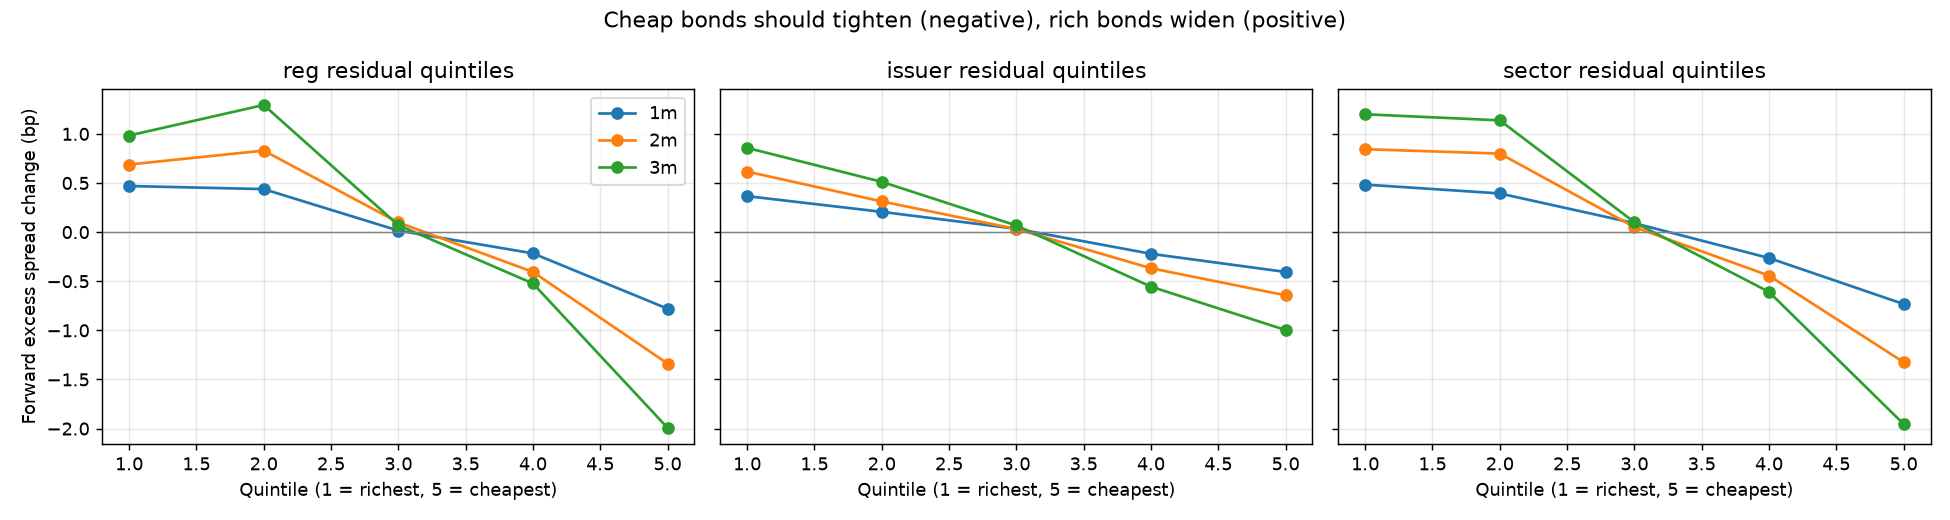
\includegraphics[width=\linewidth]{figures/backtest_quintiles.png}
\caption{Forward excess spread change by residual quintile (1 = richest, 5 = cheapest).}
\end{figure}

\textbf{Half-life.} Per-bond AR(1) fits suggest about 3 months, but with $\sim$32 observations per bond the estimate is biased toward fast reversion. Three better estimates agree on \textbf{8--12 months}: bias-corrected per-bond AR(1) 7.8 months, pooled AR(1) 8.8 months, and the share of the residual left after three months (0.84, implying 11.7 months). Most of the closing comes from the bond's own spread moving, not the model's fair value shifting. The signal is statistically robust but economically modest: a few basis points per quarter is about one bid/ask.

\section{The trade}
Candidate pairs must share sector and call structure, with workouts within 1.5 years, prices within 8 points and issue vintages within 5 years. The highest-scoring pairs were banks, but the data cannot distinguish covered bonds, deposit notes and bail-in senior, so the pitch uses the cleanest non-bank pair.

\begin{table}[h]\centering\small
\begin{tabular}{@{}lll@{}}\toprule
 & Long (cheap) & Short (rich) \\ \midrule
Bond & Pembina 3.62\% Apr-2029 & TCPL 3.00\% Sep-2029 \\
Issued & 2019 & 2019 \\
G-spread (BVAL) & 64bp & 52bp \\
Model residual (z) & +14bp (+1.8) & $-$8bp ($-$1.0) \\
Net debt / EBITDA & 3.1x & 4.4x \\
Ratings (S\&P / Moody's / DBRS) & BBB / NR / BBB (high) & BBB+ / Baa2 / BBB (high) \\
Face (CS01-neutral) & C\$10.0mm & C\$8.61mm \\ \bottomrule
\end{tabular}
\end{table}

\textbf{Thesis.} Same sector, same vintage, prices 2 points apart and maturities 5 months apart. Pembina carries much less leverage than TCPL with a similar rating, yet trades wider; the model puts the gap at 21bp after controlling for maturity, rating, size, coupon, age and structure. Legs are sized to equal CS01 (C\$2,346 per bp), which removes exposure to broad spread moves.

\textbf{Checked against Bloomberg and CIRO.} On September 30, Bloomberg BVAL put the pair's G-spread gap at 12bp and September CIRO trade prints implied 12--14bp, in line with the 13bp from the ETF data. The pricing holds up; the costs change the result.

\begin{table}[h]\centering\small
\caption{Expected 12-month P\&L (bp of relative spread)}
\begin{tabular}{@{}lrr@{}}\toprule
Component & Model & With Bloomberg costs \\ \midrule
Convergence: $21 \times (1-0.94^{12})$ & +11.2 & +11.2 \\
Carry (net of funding) & +7.9 & +7.9 \\
Roll-down & $-$5.2 & $-$5.2 \\
Bid/ask & $-$4.0 (assumed) & $-$7.3 (BVAL) \\
Repo borrow on the short ($\sim$15bp/yr) & -- & $-$5.4 \\ \midrule
\textbf{Expected} & \textbf{+9.9 ($\approx$C\$23k)} & \textbf{+1.2 ($\approx$C\$3k)} \\ \bottomrule
\end{tabular}
\end{table}

At today's 21bp gap the trade is roughly breakeven, so it is a hold rather than a buy. With the same costs, a gap of about \textbf{29bp} would be needed for +5bp over 12 months, which the pitch sets as the entry threshold. Risks: the gap has held around 20bp for a year as TC Energy cut leverage after the South Bow spin-off; Pembina is the smaller issuer and not rated by Moody's.

\begin{figure}[h]\centering
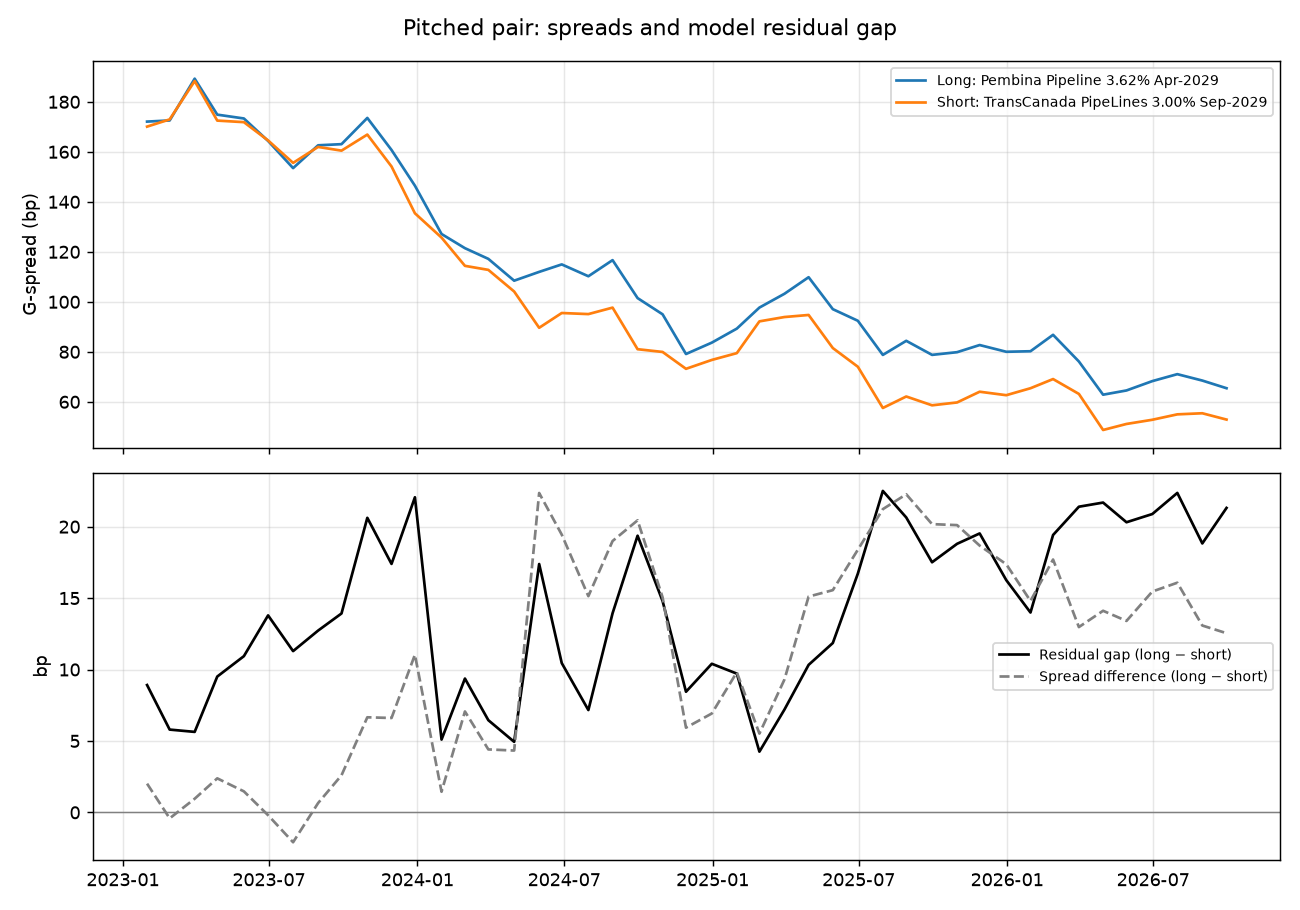
\includegraphics[width=0.85\linewidth]{figures/pair_history.png}
\caption{Pembina vs TCPL: spreads (top) and model residual gap (bottom), 2023--2026.}
\end{figure}

\section{Limitations}
\begin{itemize}[leftmargin=12pt]
  \item \textbf{Evaluated prices.} The model history uses vendor-evaluated ETF prices, which smooth gaps; only the pitched pair was checked against BVAL and CIRO.
  \item \textbf{Few issuers.} Twelve issuers in the regression (seven non-banks) can sort credit quality but not estimate the effect of leverage.
  \item \textbf{Missing inputs.} Ratings for Hydro One, Brookfield Infrastructure and National Bank (20\% of bond-months) and amounts outstanding are not yet filled.
  \item \textbf{One regime.} 45 month-ends of mostly tightening spreads.
  \item \textbf{Inferred structure.} Callables and floaters are detected from duration; bank covered, deposit-note and bail-in programs cannot be told apart.
\end{itemize}

\section{Conclusion}
A model built from public data can find relative value in Canadian investment-grade credit that persists and closes slowly. Most apparent mispricings are structural (coupon, age and call effects) and have to be removed first. The remaining signal is statistically reliable but small, and the trade analysis shows the practical lesson: real execution and financing costs decide whether a mispricing is worth trading.

\vspace{4pt}
{\small\color{gray} Tools: Python (pandas, statsmodels, SciPy, Matplotlib), Bloomberg (BVAL, YAS), CIRO bond trade data, SEC EDGAR.}

\end{document}
